The grid is composed of triangles but for simplicity these 
are obtained by splitting rectangles in two, as shown hereunder:

\begin{center}
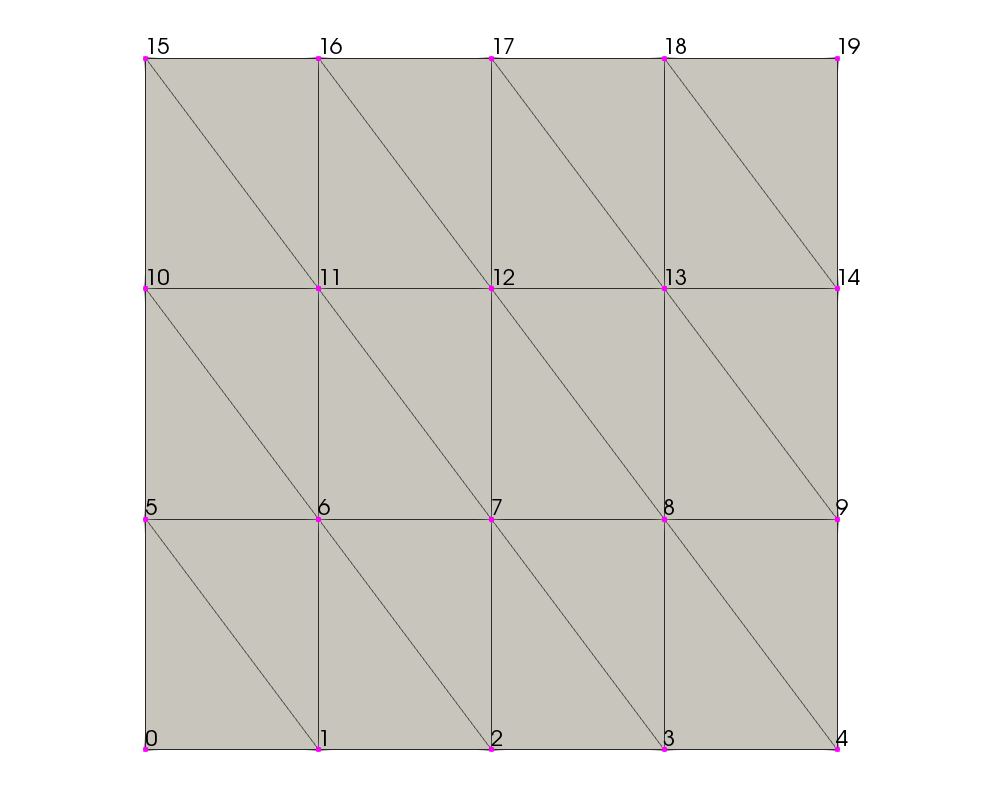
\includegraphics[width=8cm]{python_codes/fieldstone_47/images/minigrid}\\
Not shown are the nodes for the bubbles in the middle of each triangle. 
\end{center}

This stone showcases the MINI element (see Section~\ref{pair:mini})
used to solve the analytical problem "Donea \& Huerta" (see Section~\ref{mms1}).
Out of convenience the pressure is set to zero at location $(x,y)=(1,1)$, so that the 
analytical solution is now $p(x,y)=x(1-x)$. 

As an experiment I have run convergence tests for two cases: using nqel=3 
quadrature points and using nqel=6 quadrature points.
We find that the velocity and pressure errors converge depend on this crucial
parameter. 
For nqel=3 the velocity and pressure errors converge quadratically and linearly respectively
but for nqel=6 they converge as $h^2$ and $h^{1.5}$ respectively:

\begin{center}
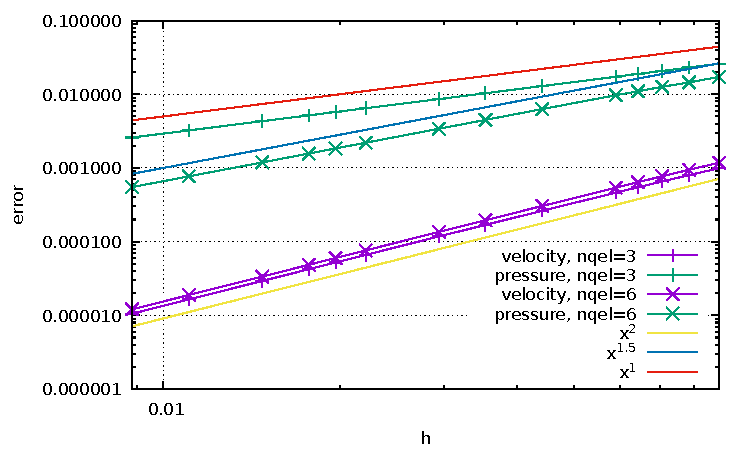
\includegraphics[width=12cm]{python_codes/fieldstone_47/images/errors}
\end{center}




